\documentclass[11pt, titlepage]{article}
\usepackage{epsfig,latexsym}
\usepackage{amsmath}
\usepackage{graphicx}
\usepackage{placeins}
\usepackage{fancyhdr}
\usepackage{listings}
\usepackage{gensymb}


\setlength{\textwidth}{7.25in}
\setlength{\textheight}{9.5in}
\setlength{\topmargin}{-0.75in}
\setlength{\oddsidemargin}{-0.5in}
\setlength{\evensidemargin}{-0.5in}
\setlength{\headheight}{26pt}

\setlength\parindent{0pt}

\lstset{
    basicstyle = \footnotesize,
    breakatwhitespace = false,
	breaklines = true,
	language = C,
	frame=single,
	tabsize=2
}

\pagestyle{fancy}
\fancyhead[R]{EEC 172 Lab5 \\
    			Richard Szeto \& Sean Ho}

\title{EEC 172 Lab5}

\author{Richard Szeto \& Sean Ho}

\date{Monday, March 18, 2013}

\begin{document}

    \maketitle
    
    \section{Objectives}
        \subsection{Part 1}
            The objective for part 1 is to control the rpm of the motor using the IR remote and display the rpm on the OLED display.
        \subsection{Part 2}
            The objective for part 2 is to calibrate the accelerometer to 2g standards and output the vector corresponding to the tilt of the accelerometer in terms of gravity.
        \subsection{Part 3}
            The objective for part 3 is to use the fast Fourier transform to manually control the rpm of the motor.
    \section{Procedures}
        \subsection{Part 1}
            We know that the rpm at 100\% duty cycle is 2190. We want to bound the output duty cycle from 10\% to 90\%. By default, we want the duty cycle to be at 50\%. Theoretically the rpm corresponding to these duty cycles are 219 rpm at 10\% duty cycle, 1095 rpm at 50\% duty cycle, and 1971 rpm for 90\% duty cycle. The IR remote will be used to to increment/decrement the duty cycle within the indicated bounds to produce the corresponding rpm of the motor.
        \subsection{Part 2}
            To calibrate the accelerometer, we modified the code that was provided in the Freescale AN3468 Application Note. After calibration, we set the appropriate offsets of the x,y, and z planes to indicate that the default tilt exhibits gravity only on the z plane.
        \subsection{Part 3}
            To transform the vibrational frequency data of the motor to a rpm, the fast Fourier transform functions provided were used. The register holding the value for the x plane was used to create the vibrational frequency data. The register was constantly being polled to produce dynamic rpm outputs.
    \section{Implementation}
        We imported most of our code from previous projects, giving us the ability to read IR signals and to easily output a PWM signal.  After that we added I2C capabilities in our initialization and added two functions that allowed us to read and write into registrars. We then copied the calibration code into our code to find the values to put in the offset registrars, however they were removed after we found the appropriate values.

    \vspace{0.5cm}
    Finally, we implemented a timer interrupt that allowed us to poll the values in the accelerometer at a rate of 125 Hz.  Every time it polls it put the data in an 128 size array.  When the array was full we would run a FFT on the dataset with the given code and put the calculated RPM in a global variable.  

    \vspace{0.5cm}
    We then added the ability for the user to add requested rpm's.  For that we  took values from the remote and stored it into an array.  After the last button was pressed, we took the string and found the rpm desired.  We would then guess the pwm value based on a ratio of the theoretical maximum values.  Then as the timer polls it would check if the calculated rpm was within 10\% of the desired rpm and if it wasn't it would increase or decrease the pwm accordingly. 
    \section{Screenshots}
        \FloatBarrier
        \begin{figure}[htbp]
            \centering
            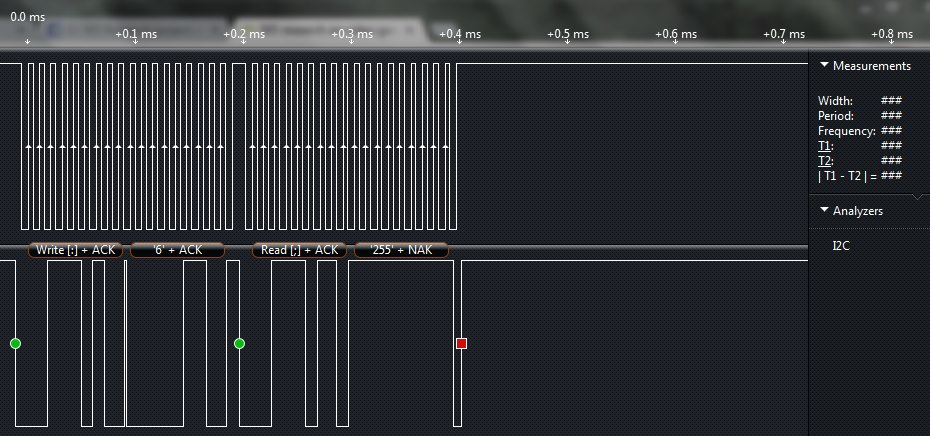
\includegraphics[scale=0.5]{Screenshot/I2C.jpg}
            \caption{An I2C transmission}
        \end{figure}
        \FloatBarrier
        
        We forgot to convert the register address into hexadecimal.
        \begin{itemize}
            \item ':' represents register 0x3A
            \item ';' represents register 0x3B 
        \end{itemize}
        From the lecture slides, we know that:
        \FloatBarrier
        \begin{figure}[htbp]
            \centering
            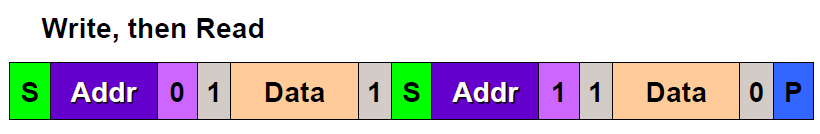
\includegraphics[scale=0.8]{Screenshot/Lecture_I2C.png}
            \caption{Write then Read in an I2C transmission}
        \end{figure}
        Corresponding to the logic analyzer screenshot, the first two dots represent the start bits and the last dot represents the stop bit. The write[0x3A] represents the address that is to be written to. The ACK following it represents that register 0x3A is ready. '6' is the data that is written to register 0x3A. The ACK following the data confirms that the data is written. The read[0x3B] represents the address that is to be read from. The ACK following it represents that register 0x3B is ready. '255' is the data that is read from register 0x3B. The NAK following it confirms that the data is read and it is the end of transmission.
    \section{Difficulties}
        \subsection{Part 1}
            Initially, we did not fully grasp how to implement the bounds of the duty cycle. When our duty cycle reached 10\%, it would still be allowed to decrease below 10\%, making the motor generate erratic behavior. The rpm would roll around from 10\% to 90\% when we tried to decrement the duty cycle below 10\%.
        \subsection{Part 2}
            When the calibration code was implemented, we did not fully understand that the calibration was only used to find the offsets. We were confused about why the values that were being output from the calibration code did not reflect our intended vector for the default tilt. Once we realized that the calibration code was only to be used as a tool for finding the offsets, the modified outputs fit our desired model.
        \subsection{Part 3}
            We had problems using the infinite while loop in main from previous labs that propagated to lab5. To find a work around, we used Timer to simulate an infinite while loop and wrote our code in the Timer interrupt that would have been in the infinite while loop.
            
            \vspace{0.5cm}
            We had trouble understanding what the fast Fourier transform functions did and what the inputs and outputs were for each of those functions. We did not understand exactly what needed to be done until we treated the functions as black boxes and analyzed the main.c that was provided with the functions. Once the vibrational frequency data was transformed into rpm, we had to allow manual control of the rpm. This brought a new problem where we needed to implement a self-correcting algorithm that will eventually produce a rpm that matched the rpm that was input from the IR remote.
    \appendix
    \section{Code for Lab5}
        \subsection{LM3S8962}
            \lstinputlisting{Code/project5_8962.c}

\end{document}

